\documentclass[10pt]{article}

\usepackage{amsmath}
\usepackage{fullpage}
\usepackage{array}
\usepackage{graphicx}
\usepackage{gensymb}
\usepackage{booktabs}
\usepackage{gensymb}
\usepackage{graphicx}
\usepackage{textcomp}
\usepackage{hyperref}
\hypersetup{colorlinks,urlcolor=blue}

\graphicspath{ {../Images/} }

\date{2014-6-22}
\pagestyle{empty}
\setlength{\parindent}{0pt}

\begin{document}
\begin{center}
\begin{Large}\textbf{Physical Science 303 - Activity}\end{Large} \\
\smallskip
%\begin{large} Acceleration \end{large}
\end{center}
%%%%%%%

\section{Archimedes' principle}
\subsection{Review}
\emph{Fluid} is a state of matter which has no fixed shape (thus it can \emph{flow}), for instance, liquid or gas.  We will be mostly dealing with the liquids.  Thus, we first review some notions used widely with liquids (or more generally with matter)
\begin{enumerate}
\item \textbf{Density}, $\rho$, is defined as the mass of the fluid (or matter) per unit volume.  Thus
  \begin{equation}
    \rho = \frac{m}{V}.
  \end{equation}
The units for density are kg/$\text{m}^3$.
Here we note that if the density $\rho$ and the volume $V$ are given we can compute the \emph{mass} by using the following equation
\begin{equation}
  m = \rho V
\end{equation}
\item \textbf{Weight} of the matter can be computed if density and volume are given 
  \begin{equation}
    \label{weigheq}
    \begin{split}
      W &= mg\\
      &= (\rho V)g
    \end{split}
  \end{equation}
where $g$ is the acceleration due to gravity (9.8 m/$\text{s}^2$) and $W$ is the weight of the given matter.  Recall that weight is a \emph{force}.
\end{enumerate}


\subsection{Activity}
\begin{enumerate}
\item \textbf{Required Box}: Box 1
\item \textbf{Required Items}: Overflow can, acrylic beaker, graduated cylinder, tap water, wooden box
\end{enumerate}
\begin{enumerate}
\item Fill up the overflow can with the tap water.  Google\textsuperscript{\texttrademark} up the density of tap water with proper units\\
$\rho_{w}:\underline{\hspace{3cm}}$ 
\item Place the acrylic beaker under the nozzle of the overflow can as shown.
\begin{figure}[h]
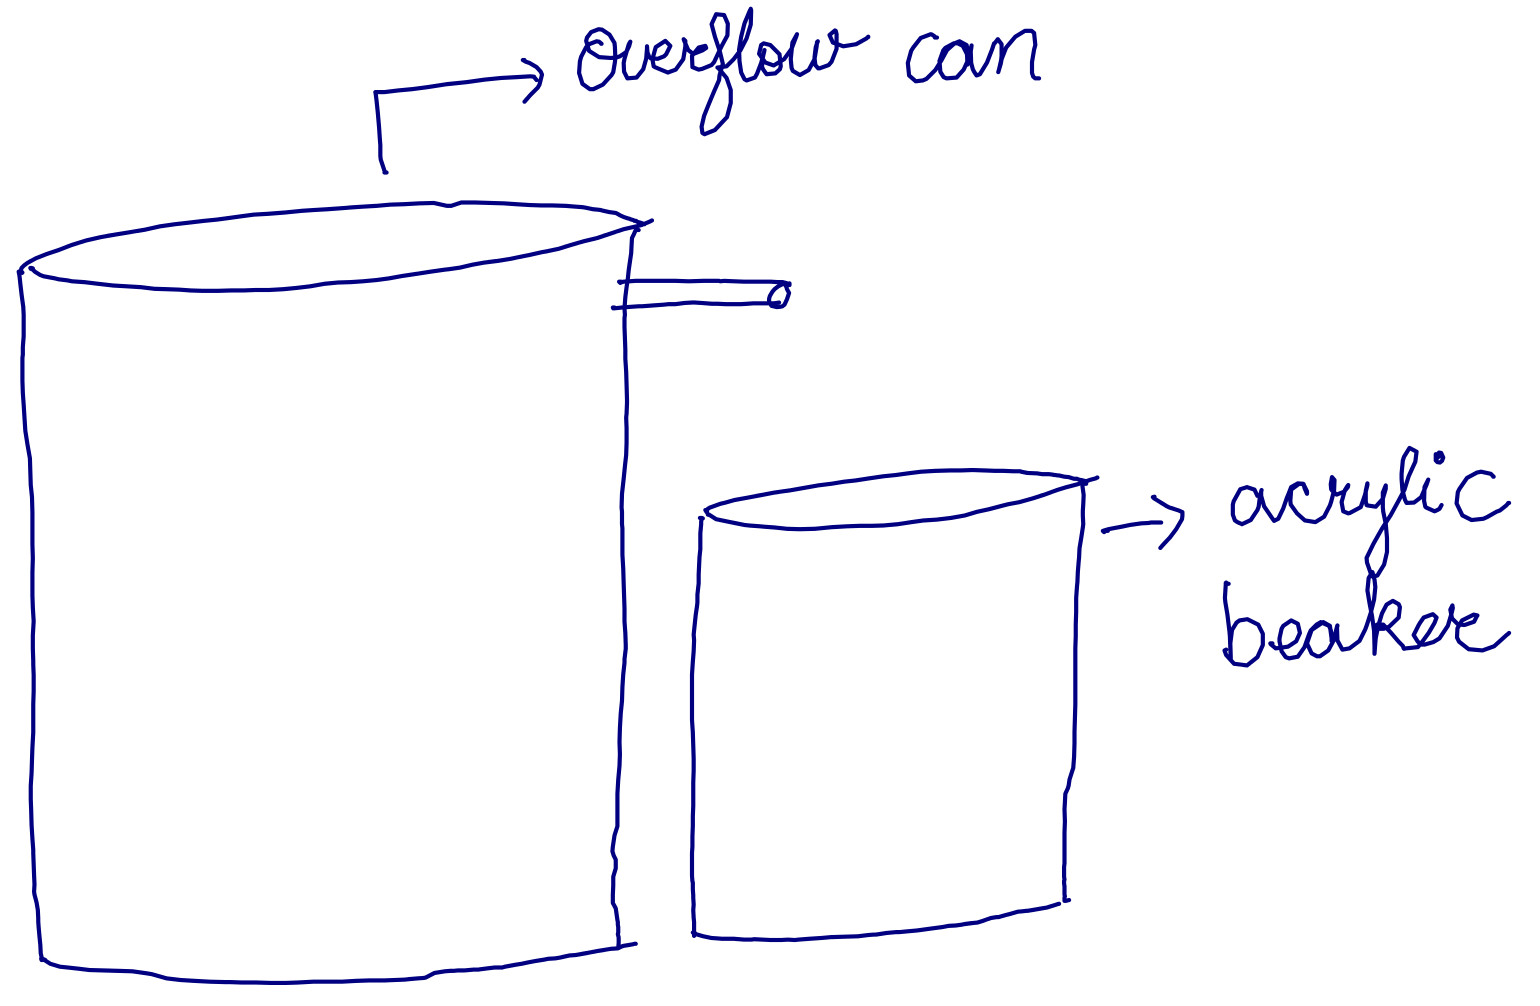
\includegraphics[scale=.3]{overflowcan}
\centering
\caption{Overflow can}
\label{pgate}
\centering
\end{figure}
\item Now immerse the wodden box in the overflow can.  You will observe some \emph{volume} of water flowing out from the nozzle into the beaker.   Write the reason for this process 
\vspace{250px}
\item Transfer the water from beaker to the graduated cylinder and measure the volume\\
$V_{\text{over}}:\underline{\hspace{3cm}}$
\item Using the equation \ref{weigheq} and density of water $\rho_{w}$, compute the weight of this displaced water
\vspace{150px}\\
$W_{\text{disp}}:\underline{\hspace{3cm}}$
\item Using pull spring or triple beam balance, measure the weight of the wodden block\\
$W_{\text{wood}}:\underline{\hspace{3cm}}$
\end{enumerate}

\subsection{Theoretical analysis}
In this section we aim to conduct the theoretical study based on the experiment.
\begin{enumerate}
\item Draw the free body diagram of the wodden box \emph{floating} in the water.  It should be useful to draw an analogy with the wodden box \emph{kept} on the table (we studied this situation earlier in the class). 
\vspace{250px}
\end{enumerate}
Here the force exerted by the water (fluid) on the wodden box is know as \emph{bouyant force}.  From the activity we conclude that the bouyant force exerted by the fluid, in the vertically upward direction, is equal to the weight of the fluid displaced by the object!  This is know as the Archimedes' principle.  I would highly encourage you to read the \href{http://www.longlongtimeago.com/once-upon-a-time/great-discoveries/eureka-the-story-of-archimedes-and-the-golden-crown/}{story}\footnote{http://www.longlongtimeago.com/once-upon-a-time/great-discoveries/eureka-the-story-of-archimedes-and-the-golden-crown} of this discovery. 

\section{Answer the following questions}
\begin{enumerate}
\item A 5 kg object is released from the rest while fully submerged in a liquid.  The liquid displaced by the submerged object has a mass of 3 kg.  How far and in what direction does the object move in 0.2 seconds, assuming that it moves freely in the liquid?
\vspace{250px}
\item Assuming that the object of volume $V$ is completely submerged in the water, does the bouyant force exerted by the water depend on the nature of the object (steel, brass, aluminium \ldots)?  Give reason for your answer.
\end{enumerate}
\end{document}
